
\vspace{-4pt}
\section{Experiments}
\label{sec:exp}

This section presents the experiments for diagnosing audio-visual shortcut reliance and evaluating targeted alignment, covering the setup (\Cref{ssec:setup}), shortcut analysis (\Cref{sec:shortcut_diagnosis}), targeted alignment improvements (\Cref{sec:alignment_tax}), and broader intervention results (\Cref{sec:beyond_temporal}).

\subsection{Experimental Setup}\label{ssec:setup}


\paragraph{Evaluation conditions and metrics.}
We evaluate audio-visual grounding under four conditions: \textit{Original}, \shift, \mute and \swap. Original videos serve as positive controls with natural audio-visual correspondence, while the interventions probe audio existence, temporal synchronization, and sound consistency. We report paired accuracy for each grounding dimension. 


\looseness-2





\paragraph{Models.}
We group evaluated models by access mode. The API-tested models include Gemini-3.1-Pro~\cite{deepmind2026gemini3}, MiMo-V2.5~\cite{xiaomi2026mimov25}, and Nemotron-3-Nano-Omni~\cite{Deshmukh2026Nemotron3N}. We also query GPT-5.5~\cite{DBLP:journals/corr/abs-2601-03267}, but omit it from~\Cref{tab:shortcut_diagnosis} because its tested interface does not support direct audio input for video; its outputs are provided in \Cref{app:gpt-qualitative}. The locally evaluated models include MiniCPM-o-4.5~\cite{Cui2026MiniCPMo4T}, Qwen3-Omni~\cite{DBLP:journals/corr/abs-2509-17765}, and Ming-flash-omni-2.0~\cite{DBLP:journals/corr/abs-2506-09344}.

\looseness-2


\paragraph{Training and general capability evaluation.}
For controlled training experiments, we use Qwen3-Omni-30B as the trainable backbone and compare checkpoints trained with different combinations of intervention data and general video data. To test whether intervention training incurs an alignment tax, we evaluate these checkpoints on Video-MME~\cite{DBLP:conf/cvpr/FuDLLRZWZSZCLLZ25}, LVBench~\cite{DBLP:journals/corr/abs-2406-08035}, DailyOmni~\cite{DBLP:journals/corr/abs-2505-17862}, and WorldSense~\cite{DBLP:journals/corr/abs-2502-04326}, which measure general video and omni-modal understanding beyond our intervention distribution. We further evaluate on VGGSoundSync~\cite{Chen21b} to test out-of-distribution temporal synchronization beyond our constructed intervention set.



\begin{table}[t]
\caption{
Paired diagnostic accuracy (\%) of video-capable multimodal models.
\textbf{Orig.} denotes naturally correlated controls, while \shift, \mute, and \swap denote counterfactual interventions.
\textbf{Avg Gap} is the average accuracy drop, reflecting shortcut reliance.
}
\label{tab:shortcut_diagnosis}
\centering
\small
\begin{tabular}{lcccccccc}
\toprule
\multirow{2}{*}{\textbf{Model}}
& \multirow{2}{*}{\textbf{Size}}
& \multicolumn{2}{c}{\textbf{Temporal Sync.}}
& \multicolumn{2}{c}{\textbf{Audio Existence}}
& \multicolumn{2}{c}{\textbf{Sound Consistency}}
& \multirow{2}{*}{\textbf{Avg Gap}} \\
\cmidrule(lr){3-4} \cmidrule(lr){5-6} \cmidrule(lr){7-8}
&
& \textbf{Orig.} & \cellcolor{shiftbg}\textbf{\shift}
& \textbf{Orig.} & \cellcolor{mutebg}\textbf{\mute}
& \textbf{Orig.} & \cellcolor{swapbg}\textbf{\swap}
&  \\
\midrule
Gemini              & N/A  & 54.9        & \cellcolor{shiftbg}46.5 & 100.0 & \cellcolor{mutebg}13.4 & 93.6 & \cellcolor{swapbg}18.3 & \cellcolor{gapbg}56.8 \\
MiniCPM-o-4.5       & 9B   & 83.8        & \cellcolor{shiftbg}13.7 & 100.0 & \cellcolor{mutebg}19.0 & 95.8 & \cellcolor{swapbg}4.9  & \cellcolor{gapbg}\textcolor{red}{80.7} \\
Nemotron-3-Omni     & 30B  & 35.9        & \cellcolor{shiftbg}26.8 & 66.2  & \cellcolor{mutebg}4.2  & 88.7 & \cellcolor{swapbg}19.9 & \cellcolor{gapbg}46.6 \\
Qwen3-Omni          & 30B  & $100.0^{*}$ & \cellcolor{shiftbg}1.4  & 95.1  & \cellcolor{mutebg}0.0  & 75.4 & \cellcolor{swapbg}37.3 & \cellcolor{gapbg}77.3 \\
Ming-Omni-2.0       & 100B & 54.2        & \cellcolor{shiftbg}20.1 & 95.7  & \cellcolor{mutebg}54.9 & 90.1 & \cellcolor{swapbg}15.5 & \cellcolor{gapbg}49.8 \\
MiMo-V2.5           & 311B & 73.9        & \cellcolor{shiftbg}9.9  & 99.3  & \cellcolor{mutebg}2.1  & 89.4 & \cellcolor{swapbg}15.3 & \cellcolor{gapbg}78.4 \\
\bottomrule
\end{tabular}
\vspace{-0.3cm}
\end{table}


\subsection{Do Video-Capable Multimodal Models Rely on Visual Shortcuts?}
\label{sec:shortcut_diagnosis}

We examine whether video-capable multimodal models verify the audio stream or infer plausible sounds from visual context. \Cref{tab:shortcut_diagnosis} reports paired diagnostic accuracy under naturally correlated \textit{Original} controls and counterfactual interventions. Original videos serve as positive controls, while drops under \shift, \mute, or \swap reveal failures when natural audio-visual correlations are broken. \textbf{Avg Gap} measures the average accuracy drop from \textit{Original} to intervention conditions, with larger values indicating a larger performance collapse under counterfactual interventions. Its formula and the LLM-judge protocol for free-form outputs are provided in \Cref{app:prompts}.


\begin{wrapfigure}[20]{r}{0.58\textwidth}
\vspace{-12pt}
\centering
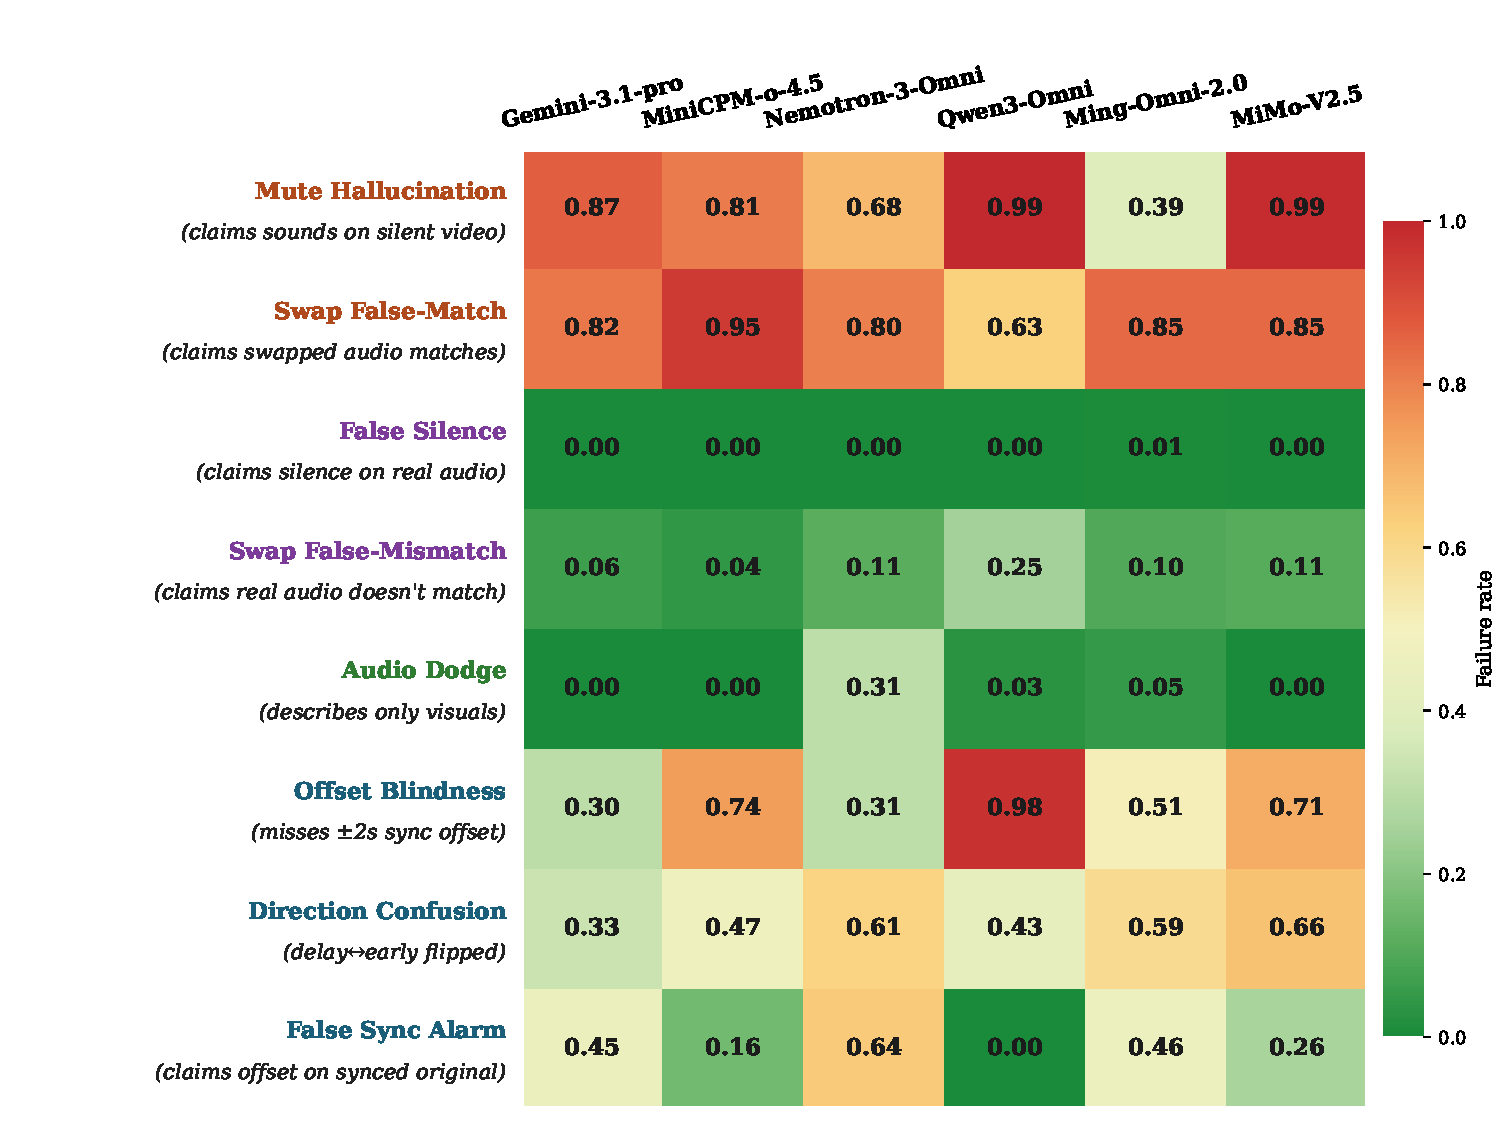
\includegraphics[width=\linewidth, trim=0 0 0 0, clip]{Fig/heatmap_v2.pdf}
\vspace{-1.5em}
\caption{
\textcolor{heatmap}{\textbf{Failure-mode heatmap}}.
Red indicates higher failure; audio hallucination dominates, while temporal failures are model-specific.
}
\label{fig:failure_heatmap}
\vspace{-0.5em}
\end{wrapfigure}


Overall, most models show large drops from \textit{Original} to intervention settings, indicating that strong performance on naturally correlated videos is fragile. MiniCPM-o-4.5 and MiMo-V2.5 have the largest gaps, 80.7\% and 78.4\%. Qwen3-Omni is diagnostic: its perfect original temporal-sync accuracy drops to 1.4\% under \shift, suggesting a synchronized-default prior rather than true temporal grounding. These results suggest that current models often rely on visual-semantic priors instead of verifying audio presence, timing, and source consistency.





\Cref{fig:failure_heatmap} exposes a uniform shortcut. Every model saturates on audio hallucination, with Mute Hallucination and Swap False-Match both above 0.63 across the board, while their symmetric counterparts (False Silence, Swap False-Mismatch) sit near zero: models invent audio that fits the visuals but rarely deny audio that is real. Temporal perception is worse. Qwen3-Omni misses 98\% of $\pm 2$\,s offsets; MiniCPM and MiMo miss roughly three quarters; and even when an offset \emph{is} flagged, the delay/early sign is wrong about half the time, close to a random label. Definitions for each axis are given in \Cref{app:failure-modes}.



\begin{figure}[b!]
\vspace{-1em}
    \centering
    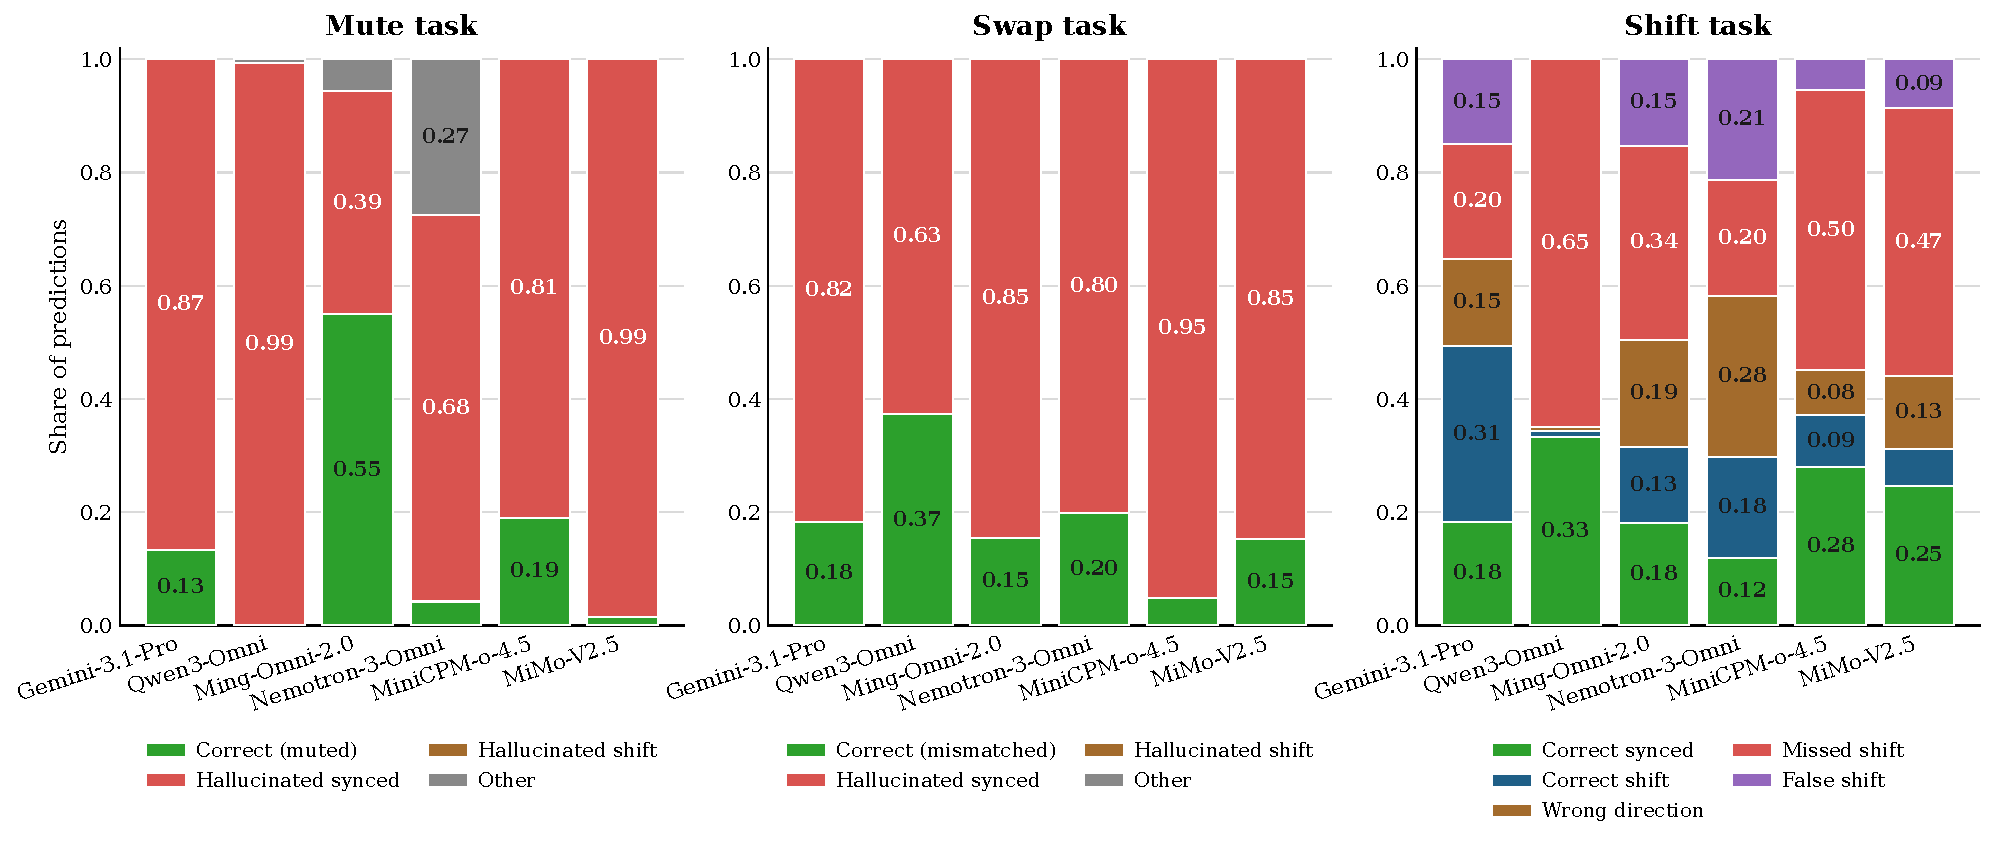
\includegraphics[width=\linewidth]{Fig/prediction_breakdown_v2.pdf}
    \vspace{-1.5em}
   \caption{
\textcolor{breakdownblue}{\textbf{Prediction breakdown}} per model on the three intervention tasks.
Errors cluster around a synced default, evidencing shortcut reliance over genuine audio-video alignment.
}
    \label{fig:breakdown}
    %\vspace{-1.6em}
    \vspace{-1em}
\end{figure}

\Cref{fig:breakdown} decomposes each model's predictions on the three intervention tasks. On Mute and Swap, almost all errors collapse onto Hallucinated synced, with five of six models fabricating matching audio on over 80\% of muted clips and the mismatched class recovered at most 37\% of the time. Hallucinated shift is negligible everywhere, indicating that models hold a strong \textit{synced} prior and rarely entertain temporal alternatives. The Shift panel makes the consequence concrete: Qwen3-Omni answers \textit{synced} on 98\% of inputs, while Gemini-3.1-Pro, Nemotron-3-Omni, and Ming-Omni-2.0 lose 19 to 22\% of predictions to Wrong direction, showing partial sensitivity to offsets without reliable sign recovery. Errors are systematically biased toward the synced prior rather than randomly distributed, indicating that current models rely on shortcut consistency rather than genuine cross-modal alignment.
\vspace{-1em}



\begin{table}[t!]
\vspace{-0.8em}
\caption{
Accuracy (\%) under different alignment recipes on temporal synchronization, general video and audio-visual understanding benchmarks. We evaluate temporal grounding on \textbf{\textcolor{syncfg}{Sync}} and \textbf{\textcolor{syncfg}{VGGSync}}, video understanding on \textbf{\textcolor{videofg}{V-MME}} and \textbf{\textcolor{videofg}{LVB}}, audio-visual understanding on \textbf{\textcolor{omnifg}{WS}} and \textbf{\textcolor{omnifg}{DO}}. \textbf{\textcolor{avgfg}{Avg.}} is the six-benchmark average. All DPO recipes are initialized from the SFT w/ OP checkpoint.
}
\vspace{3pt}

\label{tab:alignment_tax}
\centering
\small
\setlength{\tabcolsep}{5.5pt}
\renewcommand{\arraystretch}{1.05}
\begin{tabular}{lSSVVOOA}
\toprule
\textbf{Recipe}
& \multicolumn{1}{c}{\textbf{\textcolor{syncfg}{Sync}}}
& \multicolumn{1}{c}{\textbf{\textcolor{syncfg}{VGGSync}}}
& \multicolumn{1}{c}{\textbf{\textcolor{videofg}{V-MME}}}
& \multicolumn{1}{c}{\textbf{\textcolor{videofg}{LVB}}}
& \multicolumn{1}{c}{\textbf{\textcolor{omnifg}{WS}}}
& \multicolumn{1}{c}{\textbf{\textcolor{omnifg}{DO}}}
& \multicolumn{1}{c}{\textbf{\textcolor{avgfg}{Avg.}}} \\
\midrule
Qwen3-Omni-30B
& 34.3 & 36.8 & 69.2 & 49.1 & 50.3 & 68.2 & 51.3 \\
% MiniCPMo-4.5
% & 37.1 & 33.4 & 67.9 & 47.3 & \textbf{52.3} & \textbf{71.0} & 51.5 \\
SFT w/ OP
& 73.9 & -- & -- & -- & -- & -- & -- \\
SFT w/ CTP + FV-D + FV-AL
& 76.1 & 46.7 & 43.8 & 40.8 & 48.2 & 66.9 & 53.8 \\
\midrule
DPO w/ SP
& 75.4 & 55.7 & 69.3 & 50.9 & 49.8 & \textbf{69.0} & 61.7 \\
DPO w/ OP + SP
& 76.5 & 56.4 & 69.9 & 47.7 & 49.7 & 68.5 & 61.5 \\
DPO w/ SP + FV-D
& 82.2 & 55.4 & 69.1 & 51.5 & 49.8 & 68.0 & 62.7 \\
DPO w/ OP + FV-D + LV-MCQA
& 83.0 & \textbf{56.6} & 69.2 & 50.4 & 49.9 & 67.6 & 62.8 \\
DPO w/ CTP + FV-D
& 81.2 & 55.8 & 69.6 & 51.4 & 49.5 & 68.0 & 62.6 \\
DPO w/ CTP + FV-D + LV-MCQA
& 82.2 & 55.7 & 69.2 & 51.1 & 49.8 & 67.8 & 62.6 \\
DPO w/ CTP + FV-D + FV-A
& 82.6 & 55.9 & 69.1 & 50.8 & 49.9 & 67.3 & 62.6 \\
\midrule
\textbf{Ours}
& \textbf{83.1} & 56.4 & \textbf{70.1} & \textbf{52.1} & \textbf{50.3} & 67.9 & \textbf{63.3} \\
\bottomrule
\end{tabular}

\vspace{0.2em}
\footnotesize{
OP: initial original-sync preference data; SP: SFT-policy negatives; CTP: counterfactual temporal preferences; FV-* and LV-MCQA denote general video preference data.
}
\vspace{-0.5cm}
\end{table}

\subsection{Targeted Alignment Improves Temporal Grounding Without Alignment Tax}
\label{sec:alignment_tax}

\begin{wrapfigure}[18]{r}{0.60\textwidth}
\vspace{-12pt}
\centering
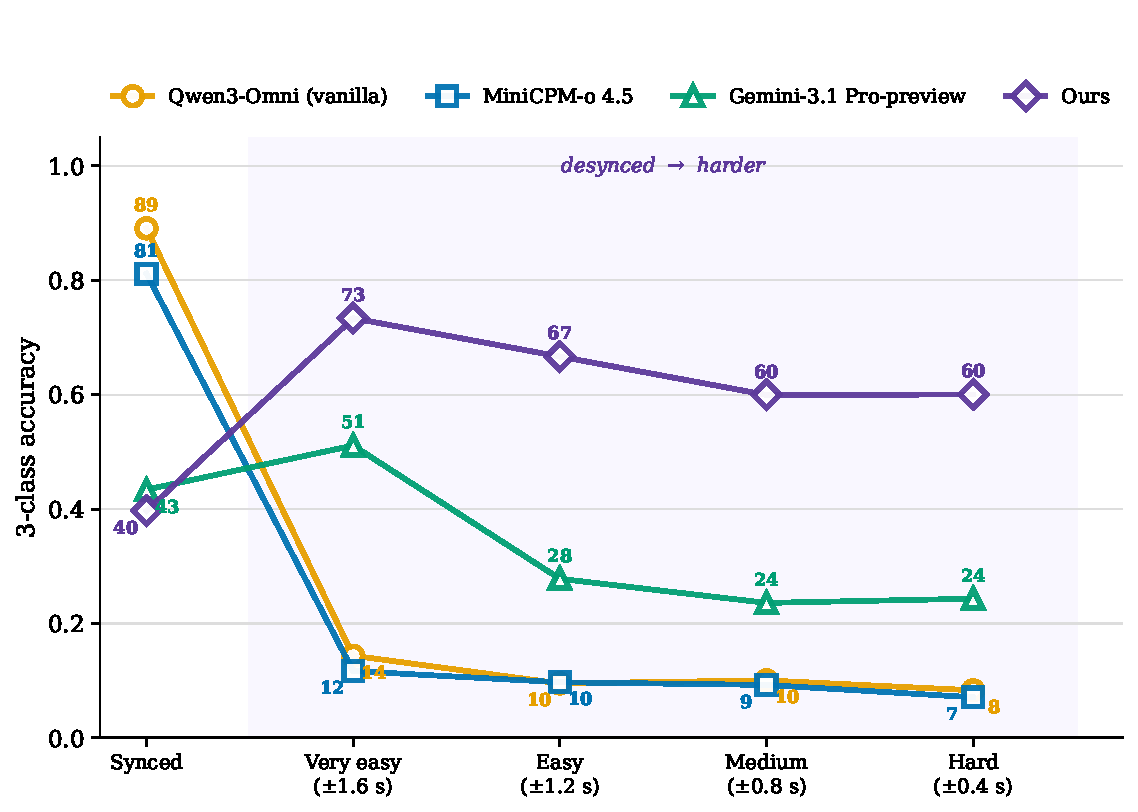
\includegraphics[width=\linewidth, trim=0 0 0 0, clip]{Fig/fig3_vgg_difficulty_curve.pdf}
\vspace{-1.5em}
\caption{
\textcolor{difficulty}{\textbf{Difficulty-band robustness}}.
Smaller offsets are harder; our model remains robust while baselines collapse under desynchronization.
}
\label{fig:vgg_diff}
\vspace{-4pt}
\end{wrapfigure}


We next ask whether targeted intervention training can improve temporal grounding without hurting general capabilities. Starting from Qwen3-Omni-30B, we compare alignment recipes using original synchronization preferences, self-sampled negatives, counterfactual temporal preferences, and general video preferences. \textbf{Ours} denotes our final 10K DPO recipe combining CTP, FV-D, and FV-A-L.~\Cref{app:recipe-data} details each data source, including its construction, preference format, and intended training signal.

\Cref{tab:alignment_tax} shows that alignment training substantially improves temporal synchronization over the vanilla Qwen3-Omni baseline. Our best 10K mixture improves \textbf{\textcolor{syncfg}{Sync}} from 34.3\% to 83.1\% and \textbf{\textcolor{syncfg}{VGGSync}} from 36.8\% to 56.4\%, suggesting that the model gains transferable temporal grounding rather than simply memorizing our intervention format. At the same time, it maintains or improves \textbf{\textcolor{videofg}{V-MME}}, \textbf{\textcolor{videofg}{LVB}}, and \textbf{\textcolor{omnifg}{WS}}, remains competitive on \textbf{\textcolor{omnifg}{DO}}, and raises the six-benchmark average accuracy from 51.3\% to 63.3\%. The contrast with the SFT-only mixture, which improves \textbf{\textcolor{syncfg}{Sync}} but sharply hurts general benchmarks, indicates that preference alignment rather than supervised mixing is key to improving temporal grounding without incurring an alignment tax.




The recipe ablation further clarifies which data sources are responsible for this tradeoff. SFT with intervention and general video data already improves \textbf{\textcolor{syncfg}{Sync}}, but substantially degrades \textbf{\textcolor{videofg}{V-MME}} and \textbf{\textcolor{videofg}{LVB}}, indicating that supervised mixing alone can over-specialize the model to intervention-style supervision. In contrast, DPO recipes recover general capability while preserving temporal gains. Self-sampled preferences provide a strong general baseline, but the best temporal results arise when targeted temporal preferences are combined with general video preference data. This suggests that counterfactual temporal supervision supplies the grounding signal, while FineVideo and LLaVA-Video preferences regularize the model toward broad video understanding.

\begin{figure*}[t!]
    \centering
    \vspace{-1em}
    \begin{subfigure}[t]{0.495\textwidth}
        \centering
        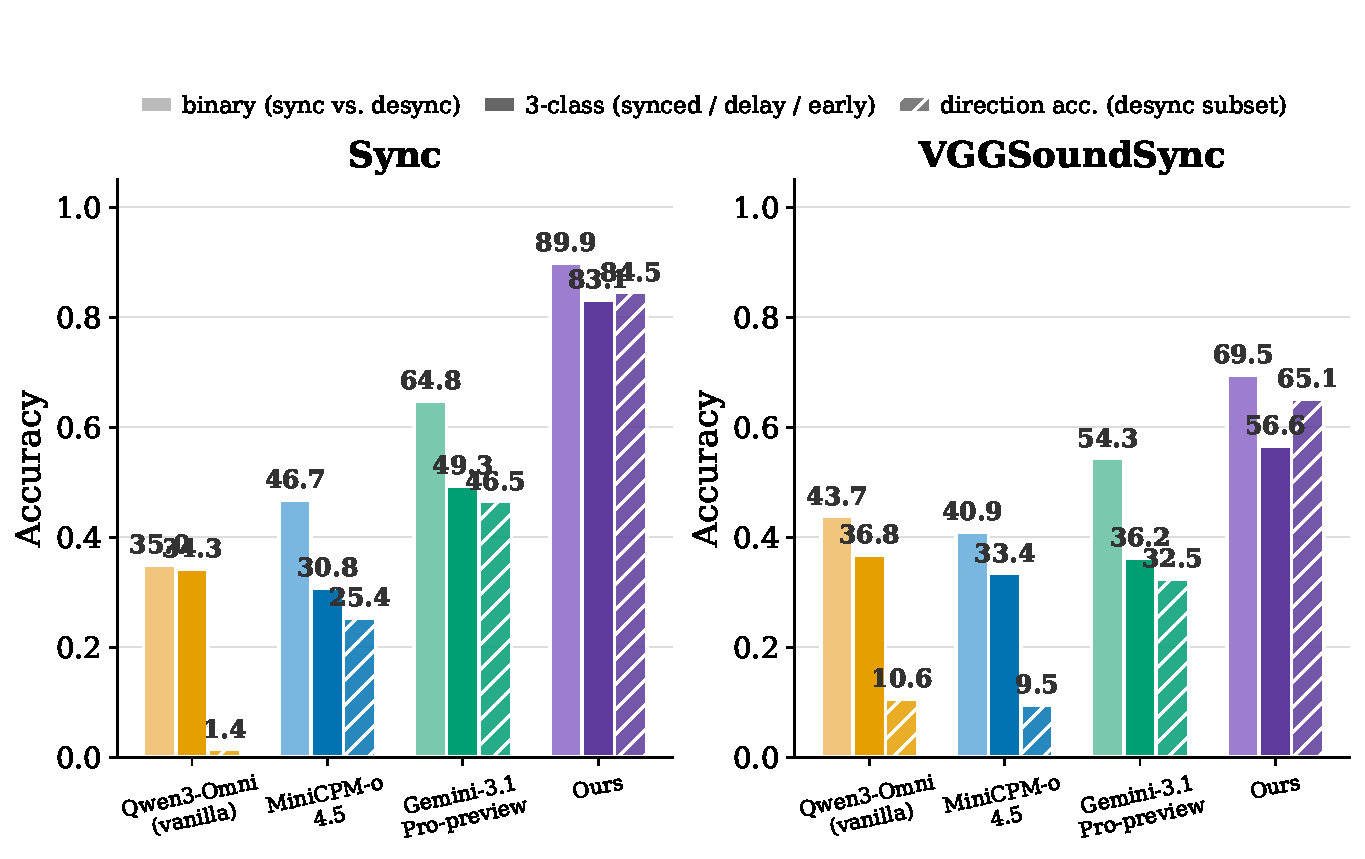
\includegraphics[width=\linewidth]{Fig/fig1_headline_accuracy.pdf}
        \caption{Audio-visual synchronization accuracy.}
        \label{fig:headline-accuracy}
    \end{subfigure}
    \hfill
    \begin{subfigure}[t]{0.495\textwidth}
        \centering
        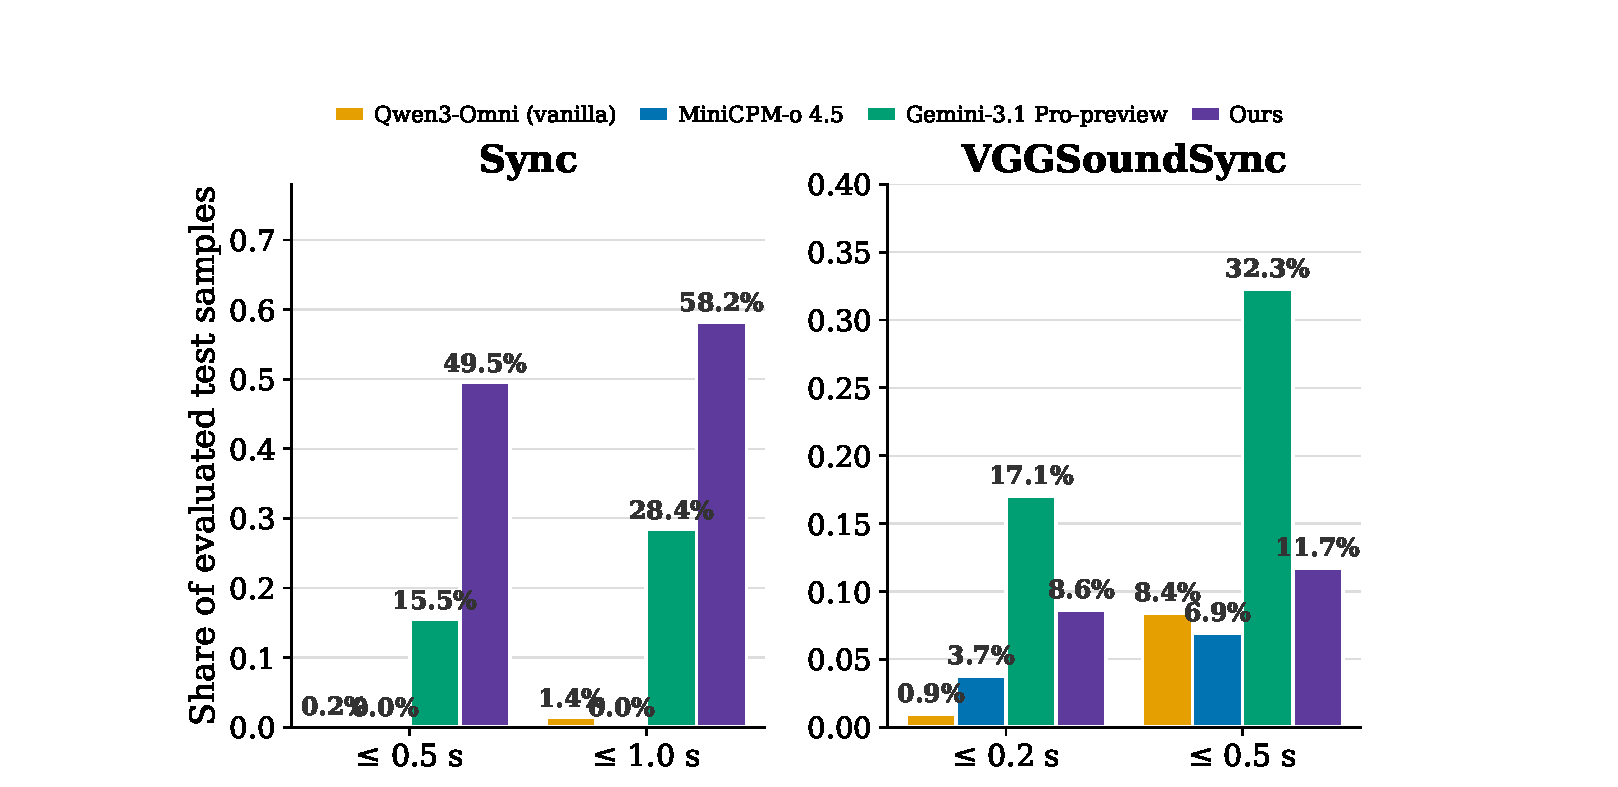
\includegraphics[width=\linewidth]{Fig/fig4_offset_coverage.pdf}
        \caption{Localization quality under offset tolerance.}
        \label{fig:offset-coverage}
    \end{subfigure}
    %\vspace{-0.5em}
    \caption{\textcolor{verifyfg}{\textbf{Complementary synchronization results.}} Left: model accuracy on binary synchronization, three-way temporal classification, and direction prediction. Right: the fraction of samples whose predicted offset is close to the ground-truth temporal displacement.}
    \label{fig:sync-results-combined}
    %\vspace{-0.8cm}
    \vspace{-1em}
\end{figure*}



\Cref{fig:vgg_diff} evaluates synchronization across temporal-offset difficulty bands on \textbf{\textcolor{syncfg}{VGGSync}}, using the \shift intervention from \Cref{sec:dspi}. Each band corresponds to a different offset magnitude $|\Delta|$. The high synced accuracy of vanilla Qwen3-Omni and MiniCPM-o should be read together with \Cref{fig:breakdown}: both models strongly prefer answering ``synced,'' making them appear accurate only when no shift is applied. Once any nonzero offset is introduced, their accuracy collapses across all bands, including large $|\Delta|$ values that should be easy to detect. Gemini-3.1-Pro follows a more expected trend, performing better on larger shifts and degrading as $|\Delta|$ becomes smaller and subtler. Our model remains stronger across all shifted bands while also reflecting the expected pattern that smaller $|\Delta|$ is harder. This suggests that temporal grounding should be judged not by synced-video accuracy alone, but by whether models show difficulty-sensitive verification under controlled audio displacement.


\begin{wrapfigure}[14]{r}{0.63\textwidth}
\vspace{-14pt}
\centering
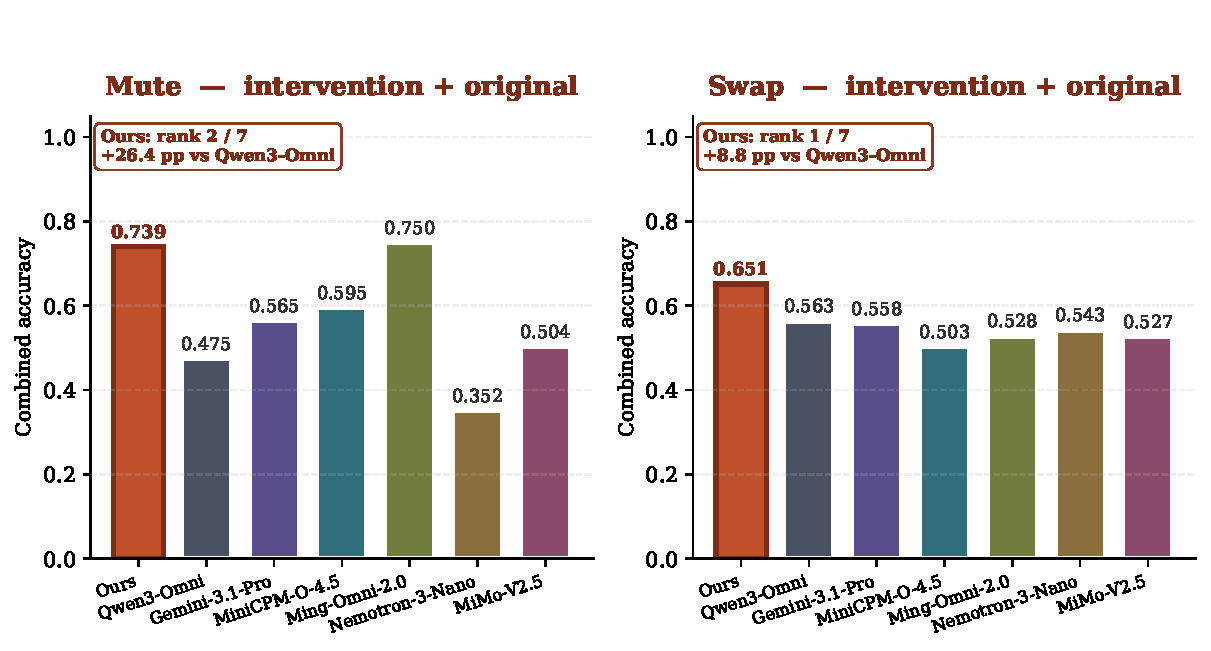
\includegraphics[width=\linewidth, trim=0 0 0 0, clip]{Fig/fig1_hero_combined_narrow.pdf}
\vspace{-1.5em}
\caption{
\textcolor{oursfg}{\textbf{Beyond temporal synchronization}}.
Combined Mute and Swap accuracy over original and intervened conditions.
}
\label{fig:beyond_sync}
\vspace{-4pt}
\end{wrapfigure}

\Cref{fig:sync-results-combined} separates temporal grounding into label-level synchronization detection and fine-grained offset localization. In \Cref{fig:headline-accuracy}, our model consistently outperforms Gemini-3.1-Pro across all synchronization metrics, including binary synced/desynced classification, three-way temporal classification, and direction prediction on desynced videos. This suggests that the improvement is not limited to coarse mismatch detection, but extends to the harder problem of identifying the temporal direction of the mismatch. \Cref{fig:offset-coverage} further sharpens this distinction: most baselines rarely predict offsets close to the ground truth, whereas our model achieves the strongest localization coverage on \textbf{\textcolor{syncfg}{Sync}} and remains competitive on \textbf{\textcolor{syncfg}{VGGSync}}. Together, these results show that audio-visual grounding should not be measured only by whether a model flags desynchronization, but also by whether it can localize the temporal mismatch with meaningful precision.




\vspace{-3pt}
\subsection{Beyond Temporal Synchronization}\label{sec:beyond_temporal}
\Cref{fig:beyond_sync} evaluates whether the recipe in \Cref{tab:alignment_tax} can extend beyond temporal synchronization. Starting from our best recipe, we add a small amount of Mute/Swap SFT. The resulting model ranks first on Swap and second on Mute, yielding a 28\% average gain over vanilla Qwen3-Omni across Shift, Mute, and Swap. \Cref{fig:falsealarm} further separates intervention detection from false alarms on original controls, showing that the gain is not merely higher combined accuracy: our model moves closer to the ideal top-left tradeoff, especially on Swap. This suggests that intervention-based training can mitigate multiple shortcut modes, while audio existence and cross-modal consistency still require targeted supervision beyond temporal alignment alone.
